
\chapter{Viscous and turbulent effects}
\section{Skin friction}
	We have already seen that the drag is caused by first the pressure distribution (form drag) and also by the viscous stresses (skin friction drag). At small $\alpha$ the skin friction represents 80-90\% of the total drag and at stall conditions it is the form drag. \\
	
	The form drag is also consequence of the viscous effects, the boundary layer due to viscous effect influences the pressure distribution. The viscous flow can be interpreted as the inviscid flow around an effective profile corrected with its boundary layer. In general this effective wing changes with $\alpha$, has a smaller camber than the real wing so that the lift curve has a smaller slope than the inviscid with $C_L$ smaller up to 10\%  for $Re = 10^6$. AC goes closer to the leading edge.   	
	
\subsection{Laminar flow}
	Consider a flat plate at $\alpha = 0$ and incompressible flow, previous courses give a skin friction of: 
	
	\begin{equation}
	C_f = \frac{1}{0.5 \rho _\infty V_\infty ^2 c} \int _0^c \tau _w \,dx = \frac{1.328}{\sqrt{Re_c}} \qquad Re_c = \frac{V_\infty c}{\nu}
	\end{equation}
	
	The boundary layer thickness $\delta$ is given by:
	
	\begin{equation}
	\delta (x) = \frac{5x}{\sqrt{Re_x}}
 	\end{equation}
 	
 	If the flow is compressible, the Mach number will play a role and the Prandtl number will appear as we have to take into account the energy equation for Navier-Stokes:
 	
 	\begin{equation}
 	Pr = \frac{\mu C_p}{\kappa}
 	\end{equation}
 	
 	In incompressible flow the temperature of the flow remained more or less constant, this is not the case here, the boundary conditions on the plate (temperature) will influence the results. The skin friction and the boundary thickness become: 
 	
 	\begin{equation}
 	C_f = \frac{1.328}{\sqrt{Re_c}}F \left( M_\infty , Pr, \frac{T_w}{T_\infty} \right)\qquad \delta = \frac{5x}{\sqrt{Re_x}}G \left( M_\infty , Pr, \frac{T_w}{T_\infty} \right)
 	\end{equation}
 	
 	 \wrapfig{8}{l}{6}{0.3}{ch4/1}{ch4/1}
 	The functions F and G are found numerically. Here are plotted for several temperature and Mach numbers the skin friction over an adiabatic flat plate. One notice that the friction decreases with temperature of the wall and with Mach number. 
 	
	\ \\ Below is plotted the effect of the temperature on the velocity field and the temperature distribution in the boundary layer. One can see that the increase of $T_w$ decreases $\frac{du}{dy}$ and so the friction $\tau _w = \mu (\frac{du}{dy})$. We also see that $\delta$ increases. On the right figure, we see that the $\delta$ increases with increasing Mach number for constant Re number. Increasing Re number decreases the friction.  
	
	\minifig{ch4/2}{ch4/3}{0.35}{0.4}{0.49}{0.49}
 	
\subsection{Turbulent flow}
	\wrapfig{8}{l}{8}{0.3}{ch4/4}{ch4/4}
	The formula now are:
	
	\begin{equation}
	C_f = \frac{0.074}{Re_c^{1/5}} \qquad \delta = \frac{0.37x}{Re_x^{1/5}}
	\end{equation}
	
	and one can see on the plot that the turbulent flow has a larger friction for the same Re and $C_f$ decreases with Mach number (the decrease is higher than laminar).

\section{Methods to reduce the drag}
\subsection{Natural laminar flow and control of laminar flow}
	As the friction in laminar flow is lower than in turbulent, one tries to keep the flow like that as possible. We have to place an active control in critical areas like the leading edge. When the air accelerates, the pressure decreases and there is a positive pressure gradient pushing from backward and leading to small separation. When the flow reataches, it becomes turbulent. This is avoided by sucking away the air in the boundary layer (slots or porous wing) as a result of what the low energy air disappears. For laminar flows, one tries to use \textbf{adapted wing profiles} and not active control. The wing profile has to be as smooth as possible and the lower pressure point as far downstream from the LE as possible. With this aim, the NACA 6 series has been developped. \\
	
	For example the NACA 65-218 has a point of min pressure at 0.5 chord downstream of the LE, the design lift coefficient 0.2 and thickness of 18\%. 
	
	\wrapfig{6}{l}{5}{0.3}{ch4/5}{ch4/5}
	On (a) is represented the pressure distribution over NACA 65-018 for design lift coefficient 0 and $c_l=0.32$. In both cases there is an undesirable pressure gradient at 50\% chord. On (b) one sees that the drag is small for $-0.3 < c_l <0.3$ $\rightarrow$ laminar. 

\ \\[5cm]
\subsection{Reduction of the drag in turbulent flows}
	\wrapfig{14}{l}{4}{0.3}{ch4/6}{ch4/6}
	An advantage of turbulent flow is that it resists better to separation, so it is preferred in reverse gradient areas. To reduce the drag, we introduce \textbf{riblets} in the flow direction.  This is illustrated on (c), the velocity distribution in the boundary layer induces spanwise vorticies in the y direction, which is unstable. Because of its instability, it is deformed and lifted away from the wall. Because of this he breaks down and induces vortices in the flow direction which desintegrate and result in turbulent flow. Riblets have a stabilizing effect, they delay the transition to turbulent and make the flow in the viscous layer less chaotic when turbulent, so reducing drag.  
	
	\ \\ 
	
	The maximum drag reduction for profile 13R is 7-8\% obtained for $s^+ \approx 15$ and 33 reduction of $\approx 2\%$. 
	\\
	
	\begin{center}
	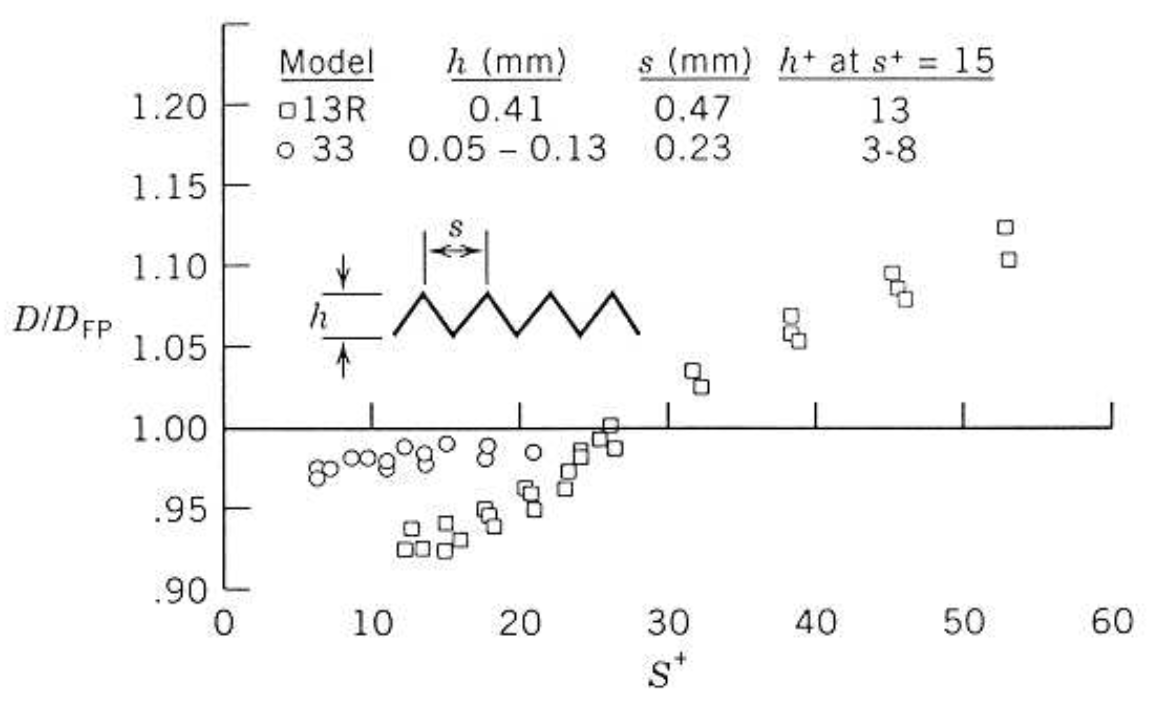
\includegraphics[scale=0.3]{ch4/7}
	\captionof{figure}{}
	\end{center}
	